\chapter{Metodologia}
Esse capítulo constará, respectivamente, com as informações técnicas referentes aos experimentos (características do computador utilizado, sistema operacional, linguagem de programação adotada, etc), os algoritmos implementados (uma breve explicação de cada um e seus respectivos códigos) e uma explicação de cada cenário analisado nesse trabalho.

\section{Informações técnicas}
Para a realização do trabalho, foi utilizado um notebook com as seguintes características:

\begin{tabular}{| r | l |}
	\hline
	\textbf{Fabricante}   & Acer \\
	\hline
	\textbf{Modelo}       & Aspire 4739 \\
	\hline
	\textbf{Placa-mãe}    & HMA CP (versão 1.08) \\
	\hline
	\textbf{Disco}        & Hitachi HTS54757 (750 GB) \\
	\hline
	\textbf{RAM}          & 8 GB \\
	\hline
	\textbf{Processador}  & Intel Core i5-480M (2.67GHz) \\
	\hline
	\textbf{Gráficos}     & Intel Ironlake Mobile \\
	\hline
	\textbf{Sistema base} & Ubuntu 16.04.2 LTS 64-bit \\
	\hline
\end{tabular}

A linguagem de programação adotada foi \textbf{C++} (\textit{C mais mais} ou \textit{C plus plus}). C++ foi escolhido devido ser considerado uma linguagem poderosa para a resolução de problemas de baixo e alto nível, prezando pela performance rápida.

O compilador usado foi o \textbf{g++}, compilador integrante da \texttt{gcc}\footnote{Originalmente escrito como compilador para o sistema operacional GNU, a \textit{GNU Compiler Collection} é um conjunto de compiladores de diversas linguagens (C, C++, Fortran, Ada, Go, etc) e é distribuído pela \textit{Free Software Foundation} (FSF). Seu site oficial é: \url{https://gcc.gnu.org/}.}. Para automatizar a compilação, fez-se uso de um arquivo \texttt{Makefile}\footnote{O arquivo Makefile define regras de compilação que serão seguidas no projeto. Ele é interpretado pelo programa \textbf{make}. A página oficial é: \url{https://www.gnu.org/software/make/}.}:

\lstinputlisting{codes/Makefile}

O editor de texto usado para escrever os códigos usados no trabalho foi o \textbf{Sublime text}\footnote{Site oficial: \url{https://www.sublimetext.com/}.}.

Para a medição de tempo, utilizou-se a biblioteca \texttt{std::chrono} do próprio \texttt{C++}, cálculando o tempo em milissegundos.

\section{Algoritmos implementados}
Nessa seção será descrito os algoritmos implementados e análisados, como também será posto seus respectivos códigos usados no projeto. Perceba que todas as funções possuem a mesma assinatura. Isso foi feito para facilitar na implementação dos códigos no projeto.

\subsection{Insertion sort}
O \textit{Insertion sort} funciona da seguinte maneira: você tem como entrada um vetor de elementos, ele irá percorrer índice por índice e a cada iteração pega aquele elemento e o coloca na posição correta, realizando as trocas necessárias com os elementos anteriores para só depois avançar na iteração. Para entender melhor, veja a imagem a seguir:

\begin{figure}[H]
	\centering
	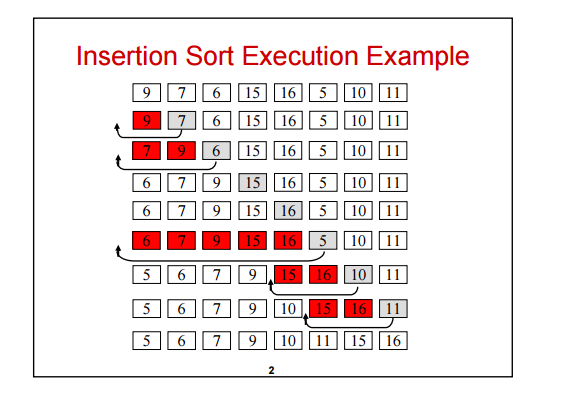
\includegraphics[scale=0.6]{img/insertion-sort.png}
	\caption{Insertion Sort.}
	\small{Imagem retirada de: \url{http://www.geeksforgeeks.org/insertion-sort/}.}
	\label{insertion-sort}
\end{figure}

Ele é considerado um algoritmo estável. Suas informações referentes a complexidade e estabilidade são:

\begin{table}[H]
 \centering
	\begin{tabular}{| r | l |}
		\hline
		\textbf{Complexidade pior caso}   & $O(n^{2})$ \\
		\hline
		\textbf{Complexidade caso médio}  & $O(n^{2})$ \\
		\hline
		\textbf{Complexidade melhor caso} & $O(n)$ \\
		\hline
	\end{tabular}
	\caption{Complexidade do Insertion Sort.}
	\label{t_insertion_sort}
\end{table}

No código a seguir, passamos como argumento o vetor que queremos ordenar. Ignoramos os outros dois parâmetros (\texttt{\_left} e \texttt{\_right}), pois eles foram colocados para apenas termos as mesmas assinaturas que as outras funções do projeto.

\lstinputlisting{codes/insertion_sort.cpp}

\subsection{Selection sort}
O \textit{Selection sort} funciona da seguinte maneira: você tem como entrada um vetor de elementos, ele irá percorrer todo o vetor atrás do menor elemento. Após percorrido, irá trocar a posição do elemento de menor valor com a posição da iteração. Assim, a cada ciclo ele garante que os elementos da posição inicial até $i-1$ ($i$ = iteração) já estejam ordenados. Para entender melhor, veja a imagem a seguir:

\begin{figure}[H]
	\centering
	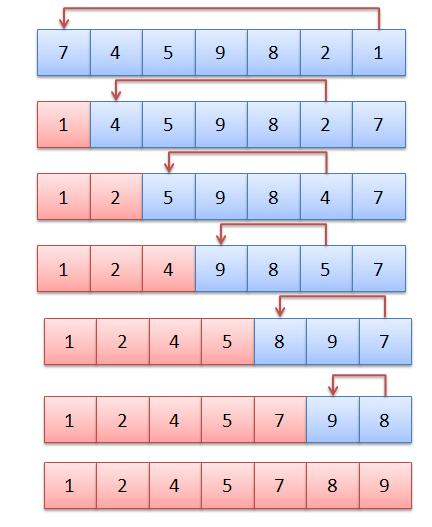
\includegraphics[scale=0.5]{img/selection-sort.jpg}
	\caption{Selection Sort.}
	\small{Imagem retirada de: \url{http://nerds-attack.blogspot.com.br/2012/09/estrutura-dados-selection-sort.html}.}
	\label{selection-sort}
\end{figure}

Suas informações referentes a complexidade são:

\begin{table}[H]
 \centering
	\begin{tabular}{| r | l |}
		\hline
		\textbf{Complexidade pior caso}   & $O(n^{2})$ \\
		\hline
		\textbf{Complexidade caso médio}  & $O(n^{2})$ \\
		\hline
		\textbf{Complexidade melhor caso} & $O(n^{2})$ \\
		\hline
	\end{tabular}
	\caption{Complexidade do Selection Sort.}
	\label{t_selection_sort}
\end{table}

No código a seguir, passamos como argumento o vetor que queremos ordenar. Ignoramos os outros dois parâmetros (\texttt{\_left} e \texttt{\_right}), pois eles foram colocados para apenas termos as mesmas assinaturas que as outras funções do projeto.

\lstinputlisting{codes/selection_sort.cpp}

\subsection{Bubble sort}
O \textit{Bubble sort} funciona da seguinte maneira: você tem como entrada um vetor de elementos, a cada iteração ele irá realizar trocas do elemento atual com os seus seguintes até encontrar a posição ideal do elemento. Para entender melhor, veja a imagem a seguir:

\begin{figure}[H]
	\centering
	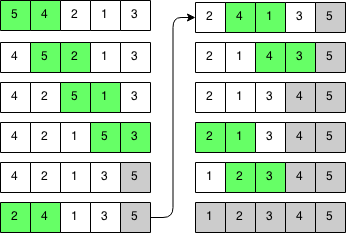
\includegraphics[scale=0.6]{img/bubble-sort.png}
	\caption{Bubble Sort.}
	\small{Imagem retirada de: \url{http://www.coisadeprogramador.com.br/algoritmos-ordenacao-bubble-sort/}.}
	\label{bubble-sort}
\end{figure}

Suas informações referentes a complexidade são:

\begin{table}[H]
 \centering
	\begin{tabular}{| r | l |}
		\hline
		\textbf{Complexidade pior caso}   & $O(n^{2})$ \\
		\hline
		\textbf{Complexidade caso médio}  & $O(n^{2})$ \\
		\hline
		\textbf{Complexidade melhor caso} & $O(n)$ \\
		\hline
	\end{tabular}
	\caption{Complexidade do Bubble Sort.}
	\label{t_bubble_sort}
\end{table}

No código a seguir, passamos como argumento o vetor que queremos ordenar. Ignoramos os outros dois parâmetros (\texttt{\_left} e \texttt{\_right}), pois eles foram colocados para apenas termos as mesmas assinaturas que as outras funções do projeto.

\lstinputlisting{codes/bubble_sort.cpp}

\subsection{Shell sort}
O \textit{Shell sort} é uma extensão do algoritmo \textit{Insertion sort}. Diferente do \textit{Selection sort} que só permite realizar trocas de elementos adjacentes, o \textit{Shell sort} permite trocas de elementos distantes um do outro. Ele funciona da seguinte maneira: você tem como entrada um vetor de elementos, usamos o tamanho desse vetor para decidir qual será a distância inicial entre os elementos que serão trocados. Após cada iteração, dividiremos a distância e assim sucessivamente até atingirmos a troca de elementos adjacentes. Para entender melhor, veja a imagem a seguir:

\begin{figure}[H]
	\centering
	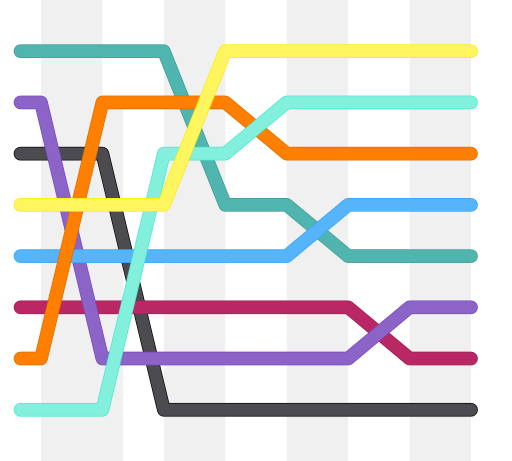
\includegraphics[scale=0.4]{img/shell-sort.png}
	\caption{Shell Sort.}
	\small{Imagem retirada de: \url{https://pt.wikipedia.org/wiki/Shell_sort}.}
	\label{shell-sort}
\end{figure}

A sua análise contêm alguns problemas matemáticos muito difíceis, por causa disso, a sua complexidade ainda não é totalmente conhecida. Suas informações referentes a complexidade até então conhecidas são:

\begin{table}[H]
 \centering
	\begin{tabular}{| r | l |}
		\hline
		\textbf{Complexidade pior caso}   & $O(nlog_{2}n)$ (melhor conhecida) \\
		\hline
		\textbf{Complexidade caso médio}  & depende da sequência da distância \\
		\hline
		\textbf{Complexidade melhor caso} & $O(n)$ \\
		\hline
	\end{tabular}
	\caption{Complexidade do Shell Sort.}
	\label{t_shell_sort}
\end{table}

No código a seguir, passamos como argumento o vetor que queremos ordenar. Ignoramos os outros dois parâmetros (\texttt{\_left} e \texttt{\_right}), pois eles foram colocados para apenas termos as mesmas assinaturas que as outras funções do projeto. Perceba que dividimos a variável `gap' em $2.2$, isso ocorre porque se a divisão der, por exemplo, $2.72727$, pegaremos apenas o valor inteiro, ou seja: $2$. Assim não teremos problemas na execução do algoritmo.

\lstinputlisting{codes/shell_sort.cpp}

\subsection{Quicksort}
O \textit{Quicksort} funciona da seguinte maneira: você tem como entrada um vetor de elementos, é então decidido um pivô e esse pivô irá dividir o vetor em duas partes (uma com números menores que ele na esquerda e outro com números maiores que ele na direita). A cada iteração, iremos aplicar essa mecânica do pivô nos subvetores, gerando outros subvetores até não conseguirmos mais gerar subvetores (vetores de 1 elemento só). Devido a essa mecânica do pivô, teremos os elementos dos subvetores organizados, logo todo o vetor original também estará organizado. Para entender melhor, veja a imagem a seguir:

\begin{figure}[H]
	\centering
	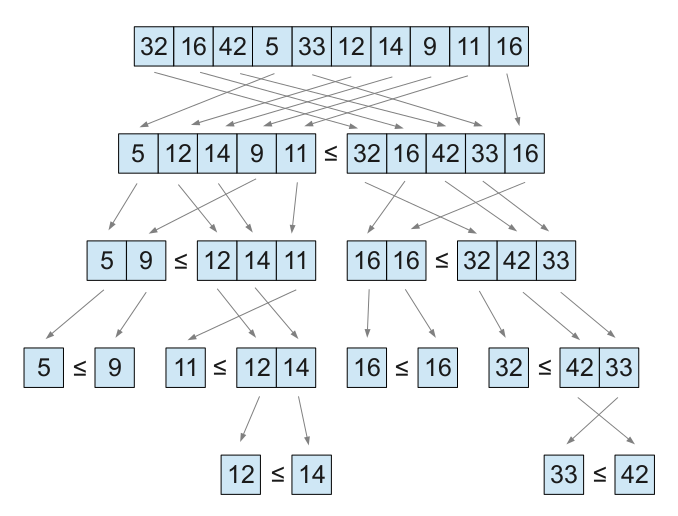
\includegraphics[scale=0.4]{img/quicksort.png}
	\caption{Quicksort.}
	\small{Imagem retirada de: \url{https://simpledevcode.wordpress.com/2014/06/13/quicksort-in-c/}.}
	\label{quicksort}
\end{figure}

Ele é considerado um algoritmo não estável. Suas informações referentes a complexidade são:

\begin{table}[H]
 \centering
	\begin{tabular}{| r | l |}
		\hline
		\textbf{Complexidade pior caso}   & $O(n^{2})$ \\
		\hline
		\textbf{Complexidade caso médio}  & $O(nlogn)$ \\
		\hline
		\textbf{Complexidade melhor caso} & $O(nlogn)$ \\
		\hline
	\end{tabular}
	\caption{Complexidade do Quicksort.}
	\label{t_quicksort}
\end{table}

No código a seguir, passamos como argumento o vetor que queremos ordenar e o índice inicial e final do vetor (respectivamente \texttt{\_left} e \texttt{\_right}). Como esse algoritmo é recursivo\footnote{Recursividade significa que uma sub-rotina (função ou método) que chama a si mesma até atingir uma condição para se encerrar.}, usamos o valor $-1$ no \texttt{\_right} para identificar sua primeira chamada.

\lstinputlisting{codes/quicksort.cpp}

\subsection{Merge sort}
O \textit{Merge sort} funciona da seguinte maneira: você tem como entrada um vetor de elementos, pegamos o indice do meio do vetor e usaremos ele para dividirmos o vetor em duas partes e usarmos o método do \textit{Merge sort} neles, até termos vetores de apenas um elemento. Nisso, iremos aplicar a função \textit{merge} do método e juntaremos esses subvetores formados pelas partes do vetor original. Para entender melhor, veja a imagem a seguir:

\begin{figure}[H]
	\centering
	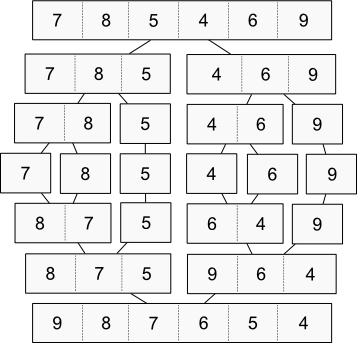
\includegraphics[scale=0.4]{img/merge_sort.png}
	\caption{Merge Sort.}
	\small{Imagem retirada de: \url{https://www.programming-algorithms.net/article/39650/Merge-sort}.}
	\label{merge_sort}
\end{figure}

Suas informações referentes a complexidade são:

\begin{table}[H]
 \centering
	\begin{tabular}{| r | l |}
		\hline
		\textbf{Complexidade pior caso}   & $\theta(nlogn)$ \\
		\hline
		\textbf{Complexidade caso médio}  & $\theta(nlogn)$ \\
		\hline
		\textbf{Complexidade melhor caso} & $\theta(nlogn)$ \\
		\hline
	\end{tabular}
	\caption{Complexidade do Merge Sort.}
	\label{t_merge_sort}
\end{table}

No código a seguir, passamos como argumento o vetor que queremos ordenar e o índice inicial e final do vetor (respectivamente \texttt{\_left} e \texttt{\_right}). Como esse algoritmo é recursivo, usamos o valor $-1$ no \texttt{\_right} para identificar sua primeira chamada. A função \textit{merge} é o que realizará a junção dos dois subvetores.

\lstinputlisting{codes/merge_sort.cpp}

\subsection{Radix sort (LSD)}
O \textit{Radix sort} funciona da seguinte maneira: você tem como entrada um vetor de elementos, a cada iteração ele irá analisar o digito do elemento, podendo começar da esquerda para a direita (\textit{MSD} - \textit{Most significant digit}, digito mais significativo) ou da direita para a esquerda (\textit{LSD} - \textit{Least significant digit}, digito menos significativo), avançando de digito a cada iteração. Para entender melhor, veja a imagem a seguir:

\begin{figure}[H]
	\centering
	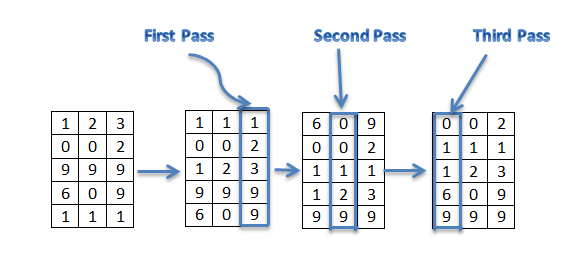
\includegraphics[scale=0.6]{img/radix_sort.png}
	\caption{Radix Sort.}
	\small{Imagem retirada de: \url{http://scanftree.com/Data_Structure/radix-sort}.}
	\label{radix-sort}
\end{figure}

Para todos os casos, ele possuirá o mesmo grau de complexidade. Suas informações referentes a complexidade são:

\begin{table}[H]
 \centering
	\begin{tabular}{| r | l |}
		\hline
		\textbf{Complexidade pior caso}   & $\theta(nk)$ \\
		\hline
		\textbf{Complexidade caso médio}  & \\
		\hline
		\textbf{Complexidade melhor caso} & \\
		\hline
	\end{tabular}
	\caption{Complexidade do Radix Sort.}
	\label{t_radix_sort}
\end{table}

No código a seguir, passamos como argumento o vetor que queremos ordenar. Ignoramos os outros dois parâmetros (\texttt{\_left} e \texttt{\_right}), pois eles foram colocados para apenas termos as mesmas assinaturas que as outras funções do projeto.

\lstinputlisting{codes/radix_sort.cpp}

\subsection{Visão geral}
A tabela a seguire, serve para se ter uma melhor visão dos graus de complexidade de cada algoritmo implementado aqui nesse trabalho.

\begin{table}[H]
 \centering
	\begin{tabular}{| r | p{2.5cm} | p{2.5cm} | p{2.5cm} |}
		\hline
		\multirow{2}{*}{textbf{Algoritmo}} & \multicolumn{3}{c|}{\textbf{Complexidade}} \\
		 & Melhor caso   & Caso médio & Pior caso \\
		\hline
		Insertion sort   & $O(n)$          & $O(n^{2})$                        & $O(n^{2})$ \\
		\hline
		Selection sort   & $O(n^{2})$      & $O(n^{2})$                        & $O(n^{2})$ \\
		\hline
		Bubble sort      & $O(n)$          & $O(n^{2})$                        & $O(n^{2})$ \\
		\hline
		Shell sort       & $O(n)$          & Depende da sequência da distância & $O(nlog_{2}n)$ (melhor conhecida) \\
		\hline
		Quicksort        & $O(nlogn)$      & $O(nlogn)$                        & $O(n^{2})$ \\
		\hline
		Merge sort       & $\theta(nlogn)$ & $\theta(nlogn)$                   & $\theta(nlogn)$ \\
		\hline
		Radix sort (LSD) &                 &                                   & $\theta(nk)$ \\
		\hline
	\end{tabular}
	\caption{Visão geral dos algoritmos de ordenação}
	\label{t_visao_geral}
\end{table}

\section{Cenários}
Foi implementado um total de 3 cenários distintos, nos quais foram aplicados os algoritmos anteriormente apresentados. Os cenários foram:

\begin{enumerate}
	\item Arranjos com elementos aleatórios;
	\item Arranjos com elementos em ordem crescente;
	\item Arranjos com elementos em ordem decrescente.
\end{enumerate}

Em todos os 3 cenários pode ocorrer de haver elementos repetidos. Eles foram aplicados nessa mesma ordem apresentada anteriormente. O mesmo arranjo é usado nos 3 cenários, pois no primeiro ele finaliza com o arranjo ordenado em ordem crescente, aí então é aplicado no segundo cenário e, após, é apenas invertido sua ordem, se tornando em um arranjo decrescente.

Para garantirmos que os cenários não se repitam durante o experimento (os números aleatórios resultarem em um arranjo crescente, por exemplo), foi escrito duas funções, uma para gerar os números aleatórios no arranjo (\texttt{new\_numbers}) e outra para validar o arranjo (\texttt{verify\_order}). O código de ambas se encontra a seguir:

\lstinputlisting{codes/arranjos.cpp}

\section{Geração de gráficos}
Foram executados 50 vezes cada um dos 3 cenários aplicando cada uma das 7 funções para cada uma das 38 entrada, totalizando 39900 registros em um arquivo \textit{CSV}\footnote{\textit{Comma-separated values}. Arquivos de texto em formato de tabela (com linhas e cada atributo na linha é separado de outro atributo por um caractere especial, normalmente ``,'' ou ``;'') usado para armazenamento de dados.}. Precisava-se, então, de gerar uma média de cada um dos cenários, em cada uma das funções e em cada uma das entradas. Para isso, utilizou-se a linguagem \texttt{Python} com a biblioteca \texttt{pandas}, os códigos foram executados no \textit{framework} \texttt{Anaconda} em um \texttt{Jupyter notebook}. O código para gerar um novo \textit{CSV} com as médias dos casos foi:

\lstinputlisting{codes/gerar_csv.py}

Foi utilizado a biblioteca \texttt{bokeh} para gerar os gráficos. Foi atribuido as seguintes cores para cada algoritmo nos gráficos:

\begin{table}[H]
 \centering
	\begin{tabular}{| r | l |}
		\hline
		\textbf{Algoritmo} & \textbf{Cor} \\
		\hline
		Insertion Sort   & Azul \\
		\hline
		Selection Sort   & Verde \\
		\hline
		Bubble Sort      & Laranja \\
		\hline
		Shell Sort       & Vermelho \\
		\hline
		Quicksort        & Roxo \\
		\hline
		Merge Sort       & Marrom \\
		\hline
		Radix sort (LSD) & Preto \\
		\hline
	\end{tabular}
	\caption{Algoritmos e suas respectivas cores nos gráficos.}
	\label{t_graph_color}
\end{table}